\documentclass[tikz,border=8pt]{standalone}
\usepackage{lmodern}
\usepackage{amsmath,amssymb,xcolor,slashed}
\usetikzlibrary{arrows.meta,decorations.markings,decorations.pathmorphing,calc}

\definecolor{qb}{HTML}{1D4E9E}   % proton (blue, like the electron line)
\definecolor{qr}{HTML}{CC3A2F}   % J/psi (red, like the muon line)
\definecolor{ttl}{HTML}{6A4FC4}  % purple titles
\definecolor{lil}{HTML}{F1E0F8}
\definecolor{lilb}{HTML}{B88AD8}
\definecolor{gry}{HTML}{555555}

\tikzset{
  qline/.style={line width=1.6pt},
  midarrow/.style={postaction={decorate,decoration={markings,
     mark=at position 0.52 with {\arrow{Stealth[length=3mm]}}}}},
  psi/.style={decorate,decoration={snake,amplitude=1.1mm,segment length=4.1mm,pre length=0pt,post length=0pt},
              line width=1.3pt,qr},
  mom/.style={-{Stealth[length=2.2mm]},gry,thin},
  vbox/.style={draw=lilb!90!black,fill=lil,rounded corners=3pt,inner sep=4pt,font=\large},
  pbox/.style={draw=gry,fill=gray!9,rounded corners=3pt,inner sep=5pt,font=\large}
}
% momentum arrow parallel to a leg, offset sideways: A, B, t1, t2, offset(cm), side, label, colour
\newcommand{\momarrow}[8]{%
  \coordinate (ma) at ($($(#1)!#3!(#2)$)!#5cm!90:(#2)$);
  \coordinate (mb) at ($($(#1)!#4!(#2)$)!#5cm!90:(#2)$);
  \draw[mom] (ma) -- (mb) node[midway,sloped,#6,inner sep=2.5pt,#8] {$#7$};
}

\begin{document}
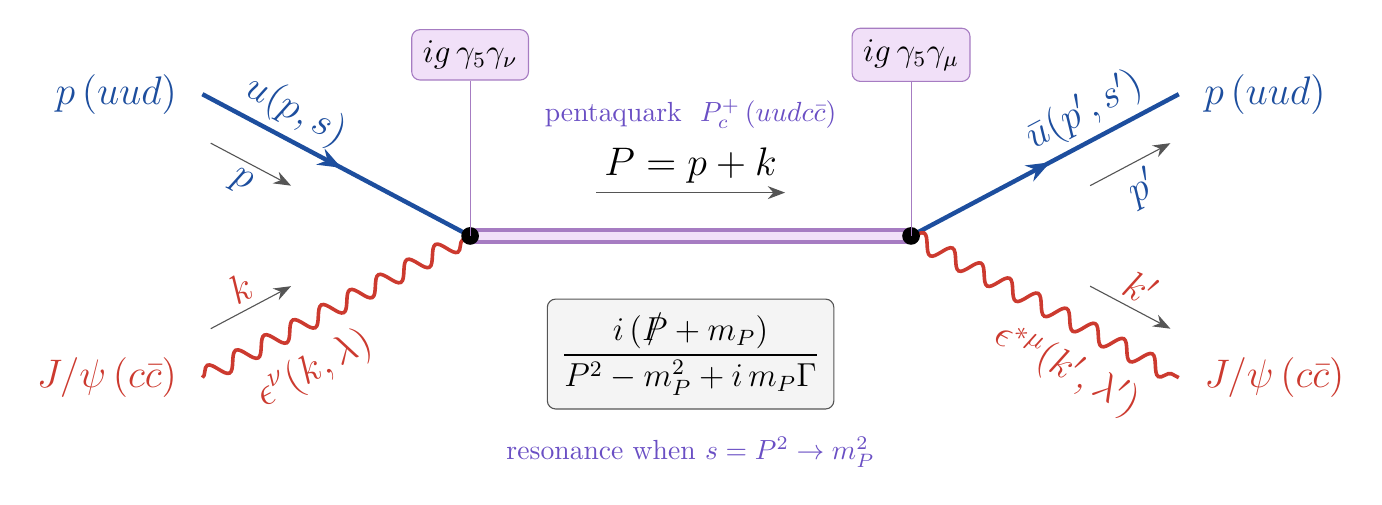
\begin{tikzpicture}[x=1cm,y=1cm,font=\Large]

\coordinate (V1) at (3.4,0);
\coordinate (V2) at (9.0,0);
\coordinate (Ai) at (0,1.8);   \coordinate (Bi) at (0,-1.8);
\coordinate (Af) at (12.4,1.8);\coordinate (Bf) at (12.4,-1.8);

% ---- pentaquark propagator: double line ----
\draw[lilb!90!black,line width=6pt,line cap=round] (V1) -- (V2);
\draw[lil,line width=3pt,line cap=round] (V1) -- (V2);

% ---- external legs ----
\draw[qb,qline,midarrow] (Ai) -- (V1);          % incoming proton
\draw[psi]               (Bi) -- (V1);          % incoming J/psi
\draw[qb,qline,midarrow] (V2) -- (Af);          % outgoing proton
\draw[psi]               (V2) -- (Bf);          % outgoing J/psi

% ---- vertices ----
\fill (V1) circle (3.2pt);
\fill (V2) circle (3.2pt);

% ---- vertex factors ----
\node[vbox] (b1) at (3.4,2.3) {$ig\,\gamma_5\gamma_\nu$};
\draw[lilb!90!black] (V1) -- (b1.south);
\node[vbox] (b2) at (9.0,2.3) {$ig\,\gamma_5\gamma_\mu$};
\draw[lilb!90!black] (V2) -- (b2.south);

% ---- spinors and polarisation vectors ----
\path (Ai) -- (V1) node[pos=0.30,sloped,above,qb,inner sep=3pt] {$u(p,s)$};
\path (Bi) -- (V1) node[pos=0.34,sloped,below,qr,inner sep=9pt] {$\epsilon^{\nu}(k,\lambda)$};
\path (V2) -- (Af) node[pos=0.70,sloped,above,qb,inner sep=3pt] {$\bar u(p',s')$};
\path (V2) -- (Bf) node[pos=0.66,sloped,below,qr,inner sep=9pt] {$\epsilon^{*\mu}(k',\lambda')$};

% ---- momenta (grey arrows, coloured labels) ----
\momarrow{Ai}{V1}{0.10}{0.40}{-0.50}{below}{p}{qb}
\momarrow{Bi}{V1}{0.10}{0.40}{0.50}{above}{k}{qr}
\momarrow{V2}{Af}{0.60}{0.90}{-0.50}{below}{p'}{qb}
\momarrow{V2}{Bf}{0.60}{0.90}{0.50}{above}{k'}{qr}

% ---- hadron names with quark content ----
\node[qb,anchor=east] at (-0.2,1.8)  {$p\,(uud)$};
\node[qr,anchor=east] at (-0.2,-1.8) {$J/\psi\,(c\bar c)$};
\node[qb,anchor=west] at (12.6,1.8)  {$p\,(uud)$};
\node[qr,anchor=west] at (12.6,-1.8) {$J/\psi\,(c\bar c)$};

% ---- intermediate pentaquark ----
\node[ttl,font=\normalsize] at (6.2,1.55) {pentaquark\ \ $P_c^+\,(uudc\bar c)$};
\draw[mom] (5.0,0.55) -- (7.4,0.55);
\node at (6.2,0.9) {$P=p+k$};

% ---- propagator box (grey, as on slide 10) ----
\node[pbox] at (6.2,-1.5) {$\dfrac{i\,(\slashed{P}+m_P)}{P^2-m_P^2+i\,m_P\Gamma}$};
\node[ttl,font=\normalsize] at (6.2,-2.75) {resonance when $s=P^2\to m_P^2$};

\end{tikzpicture}
\end{document}
